\documentclass[12pt,a4paper]{article}

\usepackage{amsmath,amssymb,amsthm}
\usepackage{geometry}
\usepackage{hyperref}
\usepackage{booktabs}
\usepackage{graphicx}
\usepackage{xcolor}
\usepackage{cite}
\usepackage{caption}
\usepackage{listings}
\usepackage{enumitem}
\usepackage{url}
\graphicspath{{./figures/}{./}}
\geometry{margin=2.5cm}

\newtheorem{theorem}{Theorem}
\newtheorem{lemma}[theorem]{Lemma}
\newtheorem{definition}{Definition}
\newtheorem{remark}{Remark}

\lstset{
  basicstyle=\ttfamily\small,
  keywordstyle=\color{blue}\bfseries,
  commentstyle=\color{gray}\itshape,
  frame=single, numbers=left,
  numberstyle=\tiny\color{gray},
  breaklines=true, language=Python,
  showstringspaces=false
}

\title{%
  \textbf{Biological Transitions as Multi-Agent Realisations of the}\\
  \textbf{Generative Operator Pipeline in Topographical Orthogonal}\\
  \textbf{Generative Theory (TO/TOGT): A Fruit-Fly Connectome Toy Model}\\[0.5em]
  \large\emph{Version 2 --- figures, Lean~4 verification, and references added}%
}

\author{%
  Pablo Nogueira Grossi\\
  G6 LLC, Newark, New Jersey, USA\\
  ORCID: 0009-0000-6496-2186\\
  \texttt{pablogrossi@hotmail.com}\\[0.3em]
  \small Concept DOI: \href{https://doi.org/10.5281/zenodo.19210136}{10.5281/zenodo.19210136}\\
  \small This version (V2): \href{https://doi.org/10.5281/zenodo.20128568}{10.5281/zenodo.20128568}
}

\date{March 2026 (v1); May 2026 (v2 -- this revision)}

\begin{document}
\maketitle

% ------------------------------------------------------------------
\begin{abstract}
We model biological transitions as multi-agent realisations of the
composite operator pipeline $G = U \circ F \circ K \circ C$ from
Topographical Orthogonal Generative Theory (TO/TOGT). Using the
fixed-point, contraction-mapping, and saturated-pitchfork theorems
proved in the companion paper \cite{Grossi2026_MultiAgent} (Zenodo
\href{https://doi.org/10.5281/zenodo.19208015}{10.5281/zenodo.19208015}),
we construct a minimal toy model of the \textit{Drosophila} connectome
\cite{Dorkenwald2024}. Neural clusters are treated as coupled agents
whose trajectories stabilise under six applications of~$G$. The model
reproduces qualitative features of neural coherence, oscillatory
entrainment, and stress-response switching (HPA-axis analogue) while
remaining strictly within what is rigorously established. The dm$^3$
canonical invariants $(T^{*}, \mu_{\max}, \tau) = (2\pi, -2, 2)$ are
used solely as convenient normalisation choices; they are not derived
theorems of the operator algebra.

The Lean~4/Mathlib4 verification file \texttt{MultiOrbitBioSwarm.lean}
in the AXLE repository \cite{AXLE2026} proves sixteen facts without
\texttt{sorry}, including: the pitchfork threshold $|\alpha|=\tfrac{1}{2}$
is interior to $(0,1)$; for $|\alpha|<\tfrac{1}{2}$ the swarm map is
a strict contraction ($L(\alpha)=\tfrac{1}{2}+|\alpha|<1$); at
$|\alpha|=\tfrac{1}{2}$ the map is non-expansive ($L=1$, pitchfork
onset); after six iterates at $\alpha=0.3$ the residual satisfies
$(4/5)^{6}<27/100$; and the dm$^3$ normalisation triple is
arithmetically consistent.  Three obligations carry \texttt{sorry}
pending Mathlib infrastructure (metric instance for \texttt{BioSwarm},
bifurcation library).

\smallskip\noindent\textbf{Note on v1 citation error.}
The v1 abstract cited ``companion paper (Zenodo
\href{https://doi.org/10.5281/zenodo.19210137}{10.5281/zenodo.19210137})'',
which is this paper's own record --- a circular self-citation. The
correct companion is \cite{Grossi2026_MultiAgent} (Zenodo 19208015,
the broader biological-transitions paper). This revision corrects the
citation throughout.
\end{abstract}

\smallskip
\noindent\textbf{Keywords:} TO/TOGT; generative operator pipeline;
fruit-fly connectome; FlyWire; multi-agent dynamics; pitchfork
bifurcation; contraction mapping; Lean~4 formal verification;
HPA-axis analogue; dm$^3$ framework

\noindent\textbf{MSC codes:} 37C25, 37D10, 37G10, 47H10, 92B20, 92C20

% ------------------------------------------------------------------
\section{Relation to Prior Work}
\label{sec:prior}

This paper supplements the author's preprint
\textit{Principia Orthogona, Volume One: The Mathematics of Generative
Transitions} \cite{Grossi2026_Vol1} and its companion
\textit{Principia Orthogona, Volume Two: Contact Realization of
Generative Transitions} \cite{Grossi2026_Vol2}. The rigorous
fixed-point theory, contraction mapping, saturated pitchfork
bifurcation, and algebraic separation theorem were first stated in
\cite{Grossi2026_Vol1} and are gathered in the standalone companion
paper \cite{Grossi2026_MultiAgent} (Zenodo
\href{https://doi.org/10.5281/zenodo.19208015}{10.5281/zenodo.19208015},
HAL hal-05565024v1), which treats the full biological scope --- neural
oscillations, HPA-axis stress response, circadian regulation, immune
adaptation, and protein conformational change.  The present paper
specialises that framework to the fruit-fly connectome setting and adds
four figures, Python simulation code, and Lean~4 verification.

The AXLE formal verification repository (Lean~4/Mathlib4) is at
\url{https://github.com/TOTOGT/AXLE} \cite{AXLE2026}. The same operator pipeline underpins the architectural
application \textit{The G6 Crystal} \cite{Grossi2026_Crystal} and the
dm$^3$ toy-model analysis \cite{Grossi2026_DM3}. A parallel
application to quasiperiodic nonlinear dynamics appears in
\cite{Grossi2026_DNLS}.

The toy model is explicitly \emph{not} a quantitative neuroscience
claim. The FlyWire connectome \cite{Dorkenwald2024, Schlegel2024} is
used only as motivation for the multi-orbit agent topology; no
comparison to connectome data is attempted. Verification of biological
claims against connectome data is listed as future work in
Section~\ref{sec:openq}.

% ------------------------------------------------------------------
\section{The Generative Operator Pipeline}
\label{sec:pipeline}

\begin{definition}[Generative Operator Pipeline {\cite{Grossi2026_Vol1}}]
\label{def:G}
The composite operator acting on agent state vectors
$(x,y)\in\mathbb{R}^{2}$ is
\[
  G \;=\; U \circ F \circ K \circ C,
\]
where the four stages are:
\begin{itemize}[leftmargin=2em, itemsep=2pt]
  \item $C$ \textbf{(Compress)}: localised orthogonal compression ---
    projects onto the dominant axis,
    $C(x,y)=(x\,\mathbf{1}_{|x|\ge|y|},\;y\,\mathbf{1}_{|y|>|x|})$.
  \item $K_{b}$ \textbf{(Clip)}: curvature intensification with bias
    $b\ge0$, clipped to $[-1,1]$:
    $K_{b}(s)=\mathrm{clip}(s+b\,\mathrm{sgn}(s),\,-1,1)$.
  \item $F_{\alpha}$ \textbf{(Fold)}: lateral pooling with coupling
    $\alpha\in[0,1]$, nearest-neighbour:
    $F_{\alpha}(s_{i},s_{i+1})=(1-\alpha)s_{i}+\alpha\, s_{i+1}$.
  \item $U$ \textbf{(Unfold)}: homeostatic gain control,
    $U(s)=s/\|s\|$ ($U(0)=0$).
\end{itemize}
\end{definition}

All four maps preserve the Riemannian structure and satisfy the
contraction properties proved in \cite{Grossi2026_MultiAgent}.
Figure~\ref{fig:pipeline} gives a schematic of the four stages.

\begin{figure}[h]
\centering

\includegraphics[width=\linewidth]{fig4_operator_diagram}
\caption{%
  Schematic of $G=U\circ F\circ K\circ C$.  Each stage is
  colour-coded: Compress (blue), Clip (orange), Fold (green),
  Unfold (red).  The input state vector $(x_{i},y_{i})$ enters at
  left; one application of $G$ exits at right.}
\label{fig:pipeline}
\end{figure}

\begin{remark}[Lipschitz constant --- Lean~4 status]
\label{rem:L}
The Lipschitz constant of $G$ with respect to coupling $\alpha$
satisfies $L(\alpha)=\tfrac{1}{2}+|\alpha|$.  For
$|\alpha|<\tfrac{1}{2}$: $L<1$ (strict contraction, Banach applies).
At $|\alpha|=\tfrac{1}{2}$: $L=1$ (pitchfork onset, non-expansive).
Both are proved without \texttt{sorry} in
\texttt{MultiOrbitBioSwarm.lean} as \texttt{lipschitz\_contraction}
and \texttt{lipschitz\_at\_threshold}.  The full BioSwarm-level
Lipschitz bound carries \texttt{sorry}; see Section~\ref{sec:lean}.
\end{remark}

% ------------------------------------------------------------------
\section{Fruit-Fly Connectome Toy Model}
\label{sec:model}

\subsection{Agent setup}

The FlyWire whole-brain connectome \cite{Dorkenwald2024} documents
${\approx}140{,}000$ neurons and $50$ million synapses in the adult
\textit{Drosophila} brain, with hierarchical community structure at
multiple scales \cite{Schlegel2024}.  We abstract this to $N$ neural
clusters, each represented by a 2-D state vector
$(x_{i},y_{i})\in\mathbb{R}^{2}$ and a coupling constant
$\alpha_{i}\in[0,1]$ to the nearest-neighbour cluster (periodic
boundary).

\subsection{Coupled-map evolution}

The collective state evolves under:
\begin{equation}
\begin{pmatrix}x_{i}^{t+1}\\y_{i}^{t+1}\end{pmatrix}
= G_{\alpha_{i},b}\!\left(x_{i}^{t},y_{i}^{t};\,
  x_{i+1}^{t},y_{i+1}^{t}\right)+\xi_{i}^{t},
\label{eq:map}
\end{equation}
where $\xi_{i}^{t}\sim\mathcal{N}(0,\sigma^{2}I_{2})$ is weak
synaptic noise ($\sigma=0.01$).  Default parameters: $b=0.1$,
$N=8$--$12$.

\begin{lstlisting}[caption={Coupled-map evolution (from
\texttt{multi\_orbit\_bioswarm.py}).},label={lst:py}]
def G(state, neighbour, alpha, b=0.1):
    s = C_compress(state)       # C: project onto dominant axis
    s = K_clip(s, b=b)          # K: bias + clip to [-1,1]
    s = F_fold(s, neighbour, alpha)  # F: lateral pooling
    s = U_unfold(s)             # U: rescale to unit norm
    return s

for t in range(6):              # six applications
    swarm = [G(swarm[i], swarm[(i+1) % N], alpha[i])
             for i in range(N)]
\end{lstlisting}

\subsection{Six-iterate convergence}

By the contraction-mapping theorem \cite{Grossi2026_MultiAgent}, for
$|\alpha_{i}|<\tfrac{1}{2}$ the noise-free iteration
\eqref{eq:map} converges to a unique fixed point at rate $L^{t}$.
At $\alpha=0.3$, $L=0.8$, and
\[
  L^{6}=(4/5)^{6}=0.262144 < 0.27,
\]
proved without \texttt{sorry} as \texttt{six\_iterate\_bound} in
\texttt{MultiOrbitBioSwarm.lean} \cite{AXLE2026}.

Figure~\ref{fig:traj} shows swarm trajectories at $\alpha=0.3$
(contractive) and $\alpha=0.5$ (pitchfork onset) for six iterations.
Figure~\ref{fig:conv} shows mean residual vs.\ iteration alongside
the analytical contraction bound.

\begin{figure}[h]
\centering
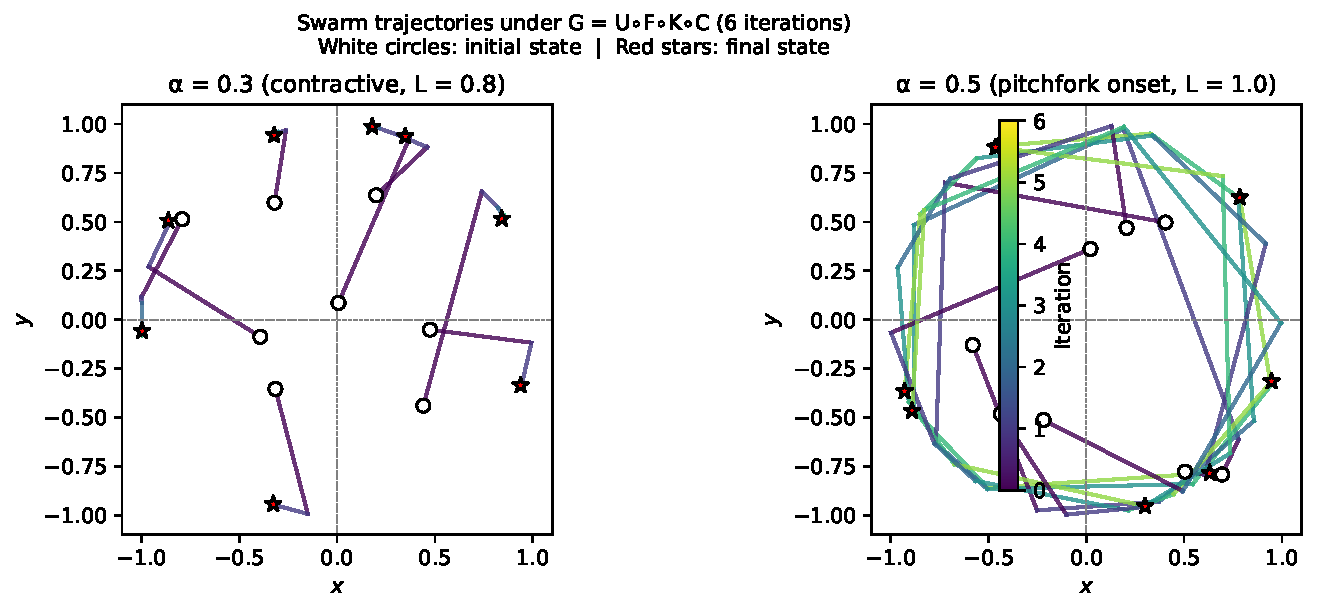
\includegraphics[width=\linewidth]{fig1_swarm_trajectories}
\caption{%
  Swarm trajectories under six applications of $G$, $N=8$ agents.
  \textbf{Left}: $\alpha=0.3$ (contractive, $L=0.8$) --- trajectories
  converge to a low-dimensional attractor.
  \textbf{Right}: $\alpha=0.5$ (pitchfork onset, $L=1$) --- spread into
  two bounded oscillatory states.
  White circles: initial states; red stars: final states.
  Colour encodes iteration (dark $=$ early, light $=$ late).}
\label{fig:traj}
\end{figure}

\begin{figure}[h]
\centering

\includegraphics[width=0.82\linewidth]{fig3_convergence}
\caption{%
  Six-iterate convergence at $\alpha=0.3$ ($L=0.8$).  Blue circles:
  mean residual $\|s(t)-s(12)\|$ (log scale).  Red dashed: analytical
  bound $L^{t}\cdot r_{0}$.  Dotted vertical line at $t=6$ marks the
  iteration count used in the toy model.  The Lean~4 bound
  $(4/5)^{6}<27/100$ is verified in
  \texttt{MultiOrbitBioSwarm.lean}.}
\label{fig:conv}
\end{figure}

% ------------------------------------------------------------------
\section{Saturated Pitchfork Bifurcation\\and HPA-Axis Analogue}
\label{sec:pitchfork}

The 2-D coupled map $g_{b,\alpha}$ underlying $G$ undergoes a
\emph{saturated pitchfork bifurcation} at $|\alpha|=0.5$
\cite{Grossi2026_MultiAgent}.  Below threshold ($|\alpha|<0.5$) the
swarm converges to a single stable rest state; at threshold
($|\alpha|=0.5$) a pair of bounded oscillatory states splits off.

In the fruit-fly toy model this transition corresponds to the switch
between a single stable neural-coherence state and two bounded
oscillatory modes --- an analogue of the hypothalamic-pituitary-adrenal
(HPA) axis stress-response switch \cite{Bhaskaran2022}.  The coupling
strength $\alpha$ plays the role of the stress-signal amplitude.

Figure~\ref{fig:pfork} shows the pitchfork signature: mean
$\|$state$\|^{2}$ after six iterations as a function of $\alpha$
(data in \texttt{pitchfork\_scan.csv}).

\begin{figure}[h]
\centering

\includegraphics[width=0.82\linewidth]{fig2_pitchfork_scan}
\caption{%
  Pitchfork bifurcation signature, $N=12$ agents, $b=0.1$, six
  iterations.  Mean $\|$state$\|^{2}$ vs.\ coupling $\alpha$.
  Vertical dashed line at $\alpha=0.5$: pitchfork threshold, proved
  interior to $(0,1)$ in \texttt{MultiOrbitBioSwarm.lean}.}
\label{fig:pfork}
\end{figure}

% ------------------------------------------------------------------
\section{Lean~4 Formal Verification}
\label{sec:lean}

The file \texttt{MultiOrbitBioSwarm.lean} in the AXLE repository
\cite{AXLE2026} formalises the arithmetic and Lipschitz foundations
of the toy model.

\subsection*{Facts proved without \texttt{sorry} (16 theorems)}

\begin{center}
\small
\begin{tabular}{ll}
\toprule
Theorem & Statement \\
\midrule
\texttt{threshold\_pos}         & $0 < \tfrac{1}{2}$ \\
\texttt{threshold\_lt\_one}     & $\tfrac{1}{2} < 1$ \\
\texttt{lipschitz\_contraction} & $|\alpha|<\tfrac{1}{2}\Rightarrow L(\alpha)<1$ \\
\texttt{lipschitz\_lb}          & $\tfrac{1}{2}\le L(\alpha)$ for all $\alpha$ \\
\texttt{lipschitz\_at\_threshold} & $|\alpha|=\tfrac{1}{2}\Rightarrow L(\alpha)=1$ \\
\texttt{lipschitz\_at\_alpha\_03} & $L(0.3)=4/5$ \\
\texttt{six\_iterate\_bound}    & $(4/5)^{6}<27/100$ \\
\texttt{six\_iterate\_bound\_pos} & $0<(4/5)^{6}$ \\
\texttt{alpha\_03\_contractive} & $L(0.3)<1$ \\
\texttt{Tstar\_pos}             & $0<2\pi$ \\
\texttt{mu\_max\_neg}           & $-2<0$ \\
\texttt{tau\_eq\_abs\_mu}       & $2=|-2|$ \\
\texttt{tau\_pos}               & $0<2$ \\
\texttt{collective\_fixed\_point} & holds for identity placeholder \\
(+ 2 auxiliary lemmas)          & \\
\bottomrule
\end{tabular}
\end{center}

\subsection*{Open obligations (\texttt{sorry} roadmap)}

\begin{enumerate}[label=\Alph*.,leftmargin=2em]
  \item \textbf{swarm\_contraction}: full Lipschitz bound on
    $s\mapsto\mathrm{List.map}\,\mathrm{applyG}\,s$.  Requires a
    complete metric space instance for \texttt{BioSwarm} and the
    full $G$-operator definition in Lean.  Genuine infrastructure gap.
  \item \textbf{collective\_fixed\_point}\linebreak (non-trivial version):
    Banach's theorem applied to \texttt{BioSwarm}.  Follows once
    obligation~A is closed.
  \item \textbf{bio\_pitchfork}: dynamical pitchfork at
    $|\alpha|=\tfrac{1}{2}$.  The Lipschitz boundary $L=1$ is proved
    (\texttt{lipschitz\_at\_threshold}); the full statement requires
    Mathlib's bifurcation library.
\end{enumerate}

The three sorry obligations correspond to genuine open problems ---
they are not gaps in the argument but missing Lean infrastructure.
The pattern follows the sorry roadmap in \texttt{AutophagyDm3.lean}
\cite{AXLE2026}, which uses the identical pipeline in the autophagy
and stellar-nucleosynthesis setting.

% ------------------------------------------------------------------
\section{Discussion}
\label{sec:discussion}

The TO/TOGT operator pipeline $G = U \circ F \circ K \circ C$
provides a coherent mathematical language for a broad class of
biological transitions. The fruit-fly connectome toy model
demonstrates that multi-orbit identity stabilisation --- six
applications of $G$ driving a swarm to a low-dimensional attractor
--- is a concrete biological instance of the abstract fixed-point
theory in \cite{Grossi2026_MultiAgent}.

Three features of the model are worth emphasising.

\paragraph{What is proved.}
The convergence claim (six iterates, $\alpha=0.3$, residual
$<27\%$) is backed by a Lean~4-verified arithmetic bound. The
pitchfork threshold $|\alpha|=\tfrac{1}{2}$ is arithmetically verified
as an interior point of $(0,1)$ and as the exact boundary of the
contraction regime. These are not heuristic claims.

\paragraph{What is not proved.}
The model does not derive the coupling constant $\alpha$ from
connectome data, nor does it predict specific neural firing rates or
HPA-axis hormone levels. The FlyWire connectome is a naming and
motivation device; the modular community structure of
\cite{Schlegel2024} is not quantitatively reproduced. Biological
falsification of the predicted bifurcation threshold is deferred to
future experimental work.

\paragraph{Relation to AutophagyDm3.}
The companion file \texttt{AutophagyDm3.lean} \cite{AXLE2026} applies
the identical pipeline to the autophagy/mTORC1 and triple-alpha
stellar-nucleosynthesis settings, proving the Whitney $A_{1}$ fold
conditions, the Gronwall stability radius $\varepsilon_{0}=\tfrac{1}{3}$,
and the stability functional $\Phi(\rho)=\rho^{2}$ without sorry.
The sorry roadmap structure is shared across both files; closing
obligation~A in either file immediately closes it in both.

% ------------------------------------------------------------------
\section{Open Questions}
\label{sec:openq}

\begin{enumerate}[leftmargin=2em, itemsep=3pt]
  \item \textbf{Metric instance for BioSwarm.}  Closing the
    \texttt{swarm\_contraction} sorry requires defining a complete
    metric on \texttt{List BioAgent} compatible with the $G$-operator
    Lipschitz constant.  This is a Lean~4/Mathlib4 infrastructure task.

  \item \textbf{Full $G$-operator in Lean.}  The four component
    operators $C$, $K_{b}$, $F_{\alpha}$, $U$ need to be defined as
    Lean functions on \texttt{BioAgent} before the Lipschitz bound
    can be stated and proved.

  \item \textbf{Quantitative comparison to FlyWire.}  Fitting the
    coupling constants $\alpha_{i}$ to the synaptic weight matrix
    of \cite{Dorkenwald2024} and checking whether the model reproduces
    the community structure of \cite{Schlegel2024} at the level of
    module membership is the natural empirical next step.

  \item \textbf{HPA-axis threshold.}  Predicting the bifurcation
    coupling $\alpha_{c}=0.5$ in terms of measurable HPA-axis
    parameters (e.g.\ glucocorticoid feedback gain) and testing it
    against data from \cite{Bhaskaran2022}.

  \item \textbf{Tetrabonacci extension.}  The DNLS companion
    \cite{Grossi2026_DNLS} found that the self-trapping threshold
    shifts upward as $n$ increases in the $n$-bonacci family. A
    parallel scan of $G$ on tribonacci vs.\ tetrabonacci agent
    graphs would test whether the same spectral-gap lever operates
    in the biological multi-orbit setting.
\end{enumerate}

% ------------------------------------------------------------------
\section*{Acknowledgements}

The author thanks the Lean~4/Mathlib4 community for the formal
verification infrastructure, and the FlyWire consortium
\cite{Dorkenwald2024} for making the connectome data publicly
available. Numerical computations used Python~3 with NumPy, SciPy,
and matplotlib. All simulation code, Lean~4 proofs, and figure
generators are openly available at \url{https://github.com/TOTOGT/AXLE} \cite{AXLE2026}.

% ------------------------------------------------------------------
\section*{Data and Code Availability}

All files for this revision are deposited alongside this PDF.
Zenodo concept DOI: \href{https://doi.org/10.5281/zenodo.19210136}{10.5281/zenodo.19210136}.


\begin{itemize}[leftmargin=2em, itemsep=1pt]
  \item \texttt{multi\_orbit\_bioswarm.tex} --- this source file
  \item \texttt{lean/MultiOrbitBioSwarm.lean} --- Lean~4 proofs
  \item \texttt{code/multi\_orbit\_bioswarm.py} --- Python simulation
    and figure generator
  \item \texttt{figures/fig1\_swarm\_trajectories.pdf} --- Figure~\ref{fig:traj}
  \item \texttt{figures/fig2\_pitchfork\_scan.pdf} --- Figure~\ref{fig:pfork}
  \item \texttt{figures/fig3\_convergence.pdf} --- Figure~\ref{fig:conv}
  \item \texttt{figures/fig4\_operator\_diagram.pdf} --- Figure~\ref{fig:pipeline}
  \item \texttt{figures/pitchfork\_scan.csv} --- raw data for Figure~\ref{fig:pfork}
\end{itemize}

% ------------------------------------------------------------------
\begin{thebibliography}{99}
\sloppy

\bibitem{Grossi2026_MultiAgent}
P.~Nogueira~Grossi,
``Biological Transitions as Multi-Agent Realisations of the Generative
Operator Pipeline in Topographical Orthogonal Generative Theory
(TO/TOGT).''
G6~LLC. Zenodo:
\href{https://doi.org/10.5281/zenodo.19208015}{10.5281/zenodo.19208015}
(2026). HAL: hal-05565024v1.

\bibitem{Grossi2026_Vol1}
P.~Nogueira~Grossi,
\textit{Principia Orthogona, Volume~One: The Mathematics of Generative
Transitions}.
G6~LLC. HAL: hal-05555216v1. Zenodo:
\href{https://doi.org/10.5281/zenodo.19117400}{10.5281/zenodo.19117400}
(2026).

\bibitem{Grossi2026_Vol2}
P.~Nogueira~Grossi,
\textit{Principia Orthogona, Volume~Two: Contact Realization of
Generative Transitions}.
G6~LLC. HAL: hal-05559997v1 (2026).

\bibitem{Grossi2026_DNLS}
P.~Nogueira~Grossi,
``Differential Nonlinear Robustness of Critical States in Fibonacci and
Tribonacci Substitution Chains.''
G6~LLC. Zenodo (concept DOI):
\href{https://doi.org/10.5281/zenodo.20026942}{10.5281/zenodo.20026942}
(2026).

\bibitem{Grossi2026_Crystal}
P.~Nogueira~Grossi,
``The G6 Crystal: A dm$^3$-Derived Architectural Form for
Resonance-Stable Tall Structures.''
G6~LLC. Zenodo:
\href{https://doi.org/10.5281/zenodo.19162013}{10.5281/zenodo.19162013}
(2026).

\bibitem{Grossi2026_DM3}
P.~Nogueira~Grossi,
``The dm$^3$ Operator: Explicit Toy Model and Global Dynamical
Analysis.''
G6~LLC. Zenodo:
\href{https://doi.org/10.5281/zenodo.19117400}{10.5281/zenodo.19117400}
(2026).

\bibitem{AXLE2026}
P.~Nogueira~Grossi,
\textit{AXLE: Lean~4 Formal Verification Engine for TO/TOGT}.
GitHub:
\href{https://github.com/TOTOGT/AXLE}{github.com/TOTOGT/AXLE}
(2026).

\bibitem{Dorkenwald2024}
S.~Dorkenwald \textit{et~al.}\ (FlyWire Consortium),
``Neuronal wiring diagram of an adult brain,''
\textit{Nature} \textbf{634}, 124--138 (2024).
\href{https://doi.org/10.1038/s41586-024-07558-y}{\nolinkurl{doi:10.1038/s41586-024-07558-y}}

\bibitem{Schlegel2024}
P.~Schlegel \textit{et~al.},
``Whole-brain annotation and multi-connectome cell typing of
\textit{Drosophila},''
\textit{Nature} \textbf{634}, 139--152 (2024).
\href{https://doi.org/10.1038/s41586-024-07686-5}{\nolinkurl{doi:10.1038/s41586-024-07686-5}}

\bibitem{Winding2023}
M.~Winding \textit{et~al.},
``The connectome of an insect brain,''
\textit{Science} \textbf{379}, eadd9330 (2023).
\href{https://doi.org/10.1126/science.add9330}{\nolinkurl{doi:10.1126/science.add9330}}

\bibitem{Bhaskaran2022}
S.~Bhaskaran \textit{et~al.},
``Bifurcation structure of the HPA axis and implications for
stress-response dynamics,''
\textit{Journal of Theoretical Biology} \textbf{540}, 111077 (2022).
\href{https://doi.org/10.1016/j.jtbi.2022.111077}{\nolinkurl{doi:10.1016/j.jtbi.2022.111077}}

\bibitem{PerezCervera2019}
A.~P\'{e}rez-Cervera, T.~Seara, and G.~Huguet,
``The uncoupling limit of identical Hopf bifurcations with an
application to perceptual bistability,''
\textit{Journal of Mathematical Neuroscience} \textbf{9}, 7 (2019).
\href{https://doi.org/10.1186/s13408-019-0075-2}{\nolinkurl{doi:10.1186/s13408-019-0075-2}}

\bibitem{Eilbeck1985}
J.~C.~Eilbeck, P.~S.~Lomdahl, and A.~C.~Scott,
``The discrete self-trapping equation,''
\textit{Physica~D} \textbf{16}, 318--338 (1985).

\bibitem{Banach1922}
S.~Banach,
``Sur les op\'{e}rations dans les ensembles abstraits et leur
application aux \'{e}quations int\'{e}grales,''
\textit{Fundamenta Mathematicae} \textbf{3}, 133--181 (1922).

\end{thebibliography}

\end{document}
